\section{introduction}
\label{submission}

\begin{figure}[ht]
  \vskip 0.2in
  \begin{center}
  \centerline{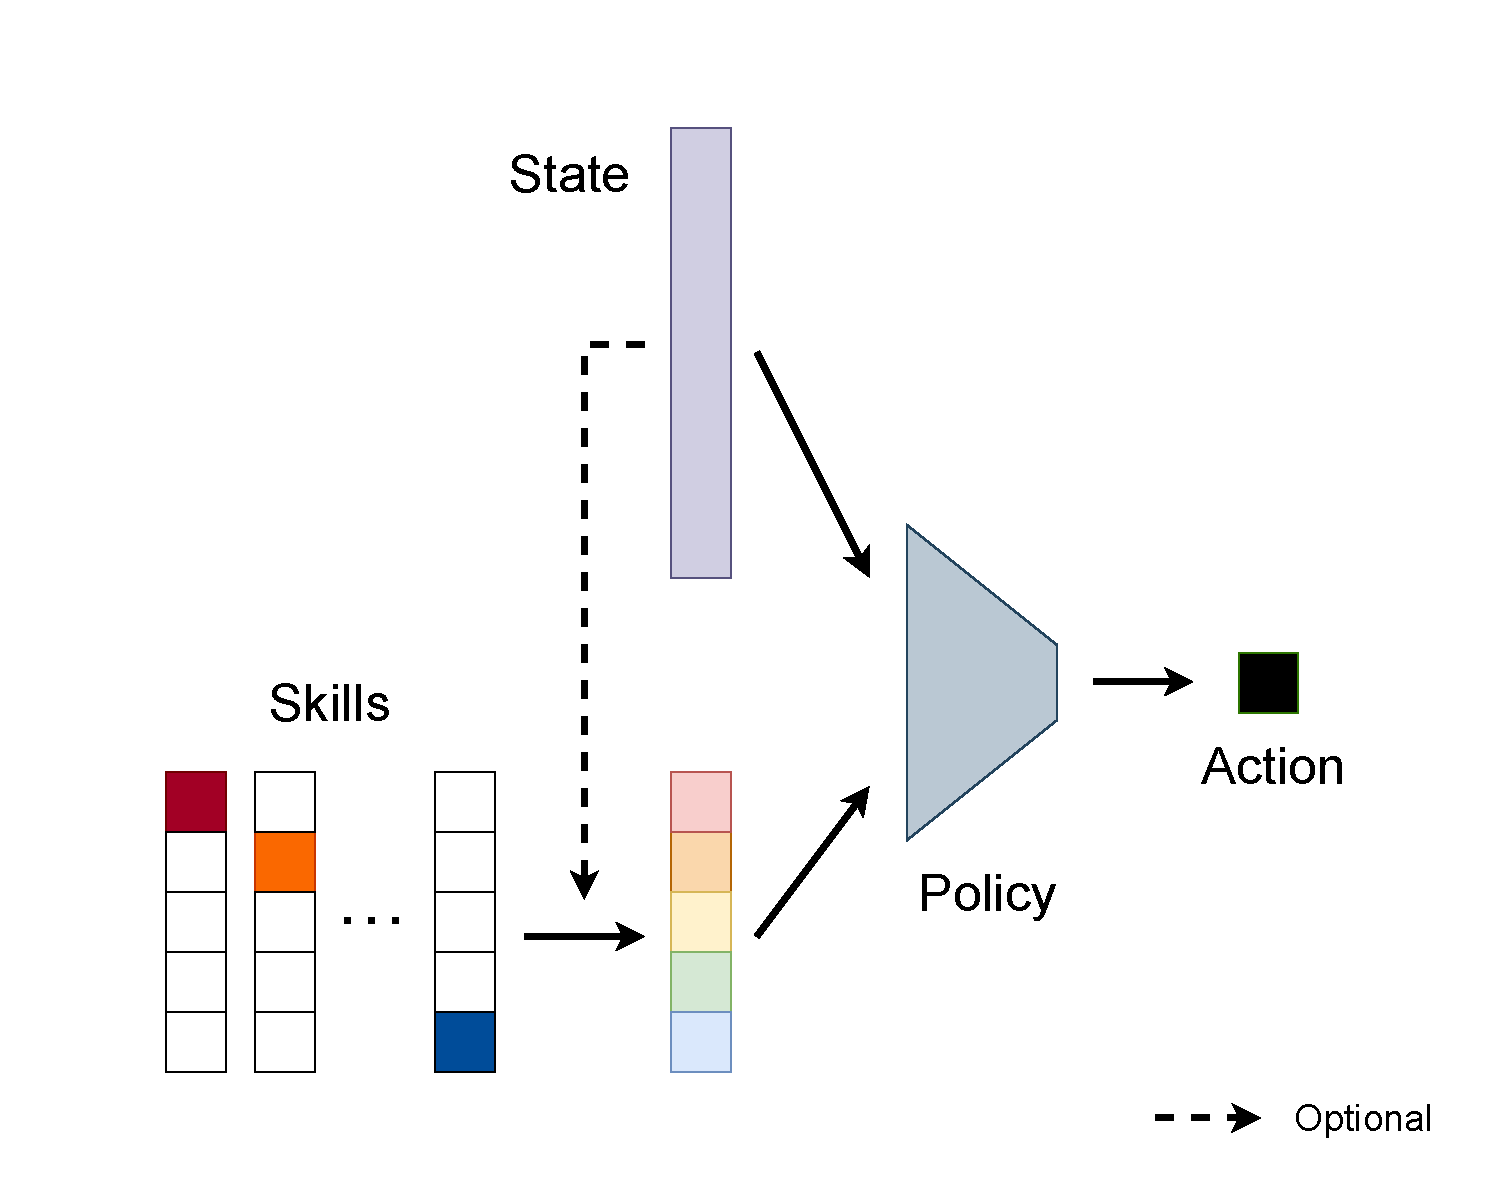
\includegraphics[width=\columnwidth]{Figures/figure_diagram.pdf}}
  \caption{Overview of methods to mix a set of learned skills in fine-tuning phase. It is optional whether the current state affects how the skills combine together.}
  \label{overview}
  \end{center}
  \vskip -0.2in
\end{figure}

Unsupervised learning for deep reinforcement learning (DRL) is challenging in the sense that an agent should interact with the world and collect data to obtain useful information without explicit reward.
In the pretraining step, an agent gathers information from the environment and learns representations of visited states, dynamics, and behaviors.
When the downstream tasks are given, the agent has to quickly adapt to them leveraging those representations.
Recent works have shown that skill discovery is a promising way to learn diverse behaviors which potentially help the agent achieve a goal \cite{salge2014empowerment, gregor2016variational, eysenbach2018diversity}.

Although the agent could learn diverse skills, it is not obvious at a glance how the agent manages them to solve a downstream task since the agent has to efficiently and effectively handle multiple policies while the agent has just one policy to control in a typical reinforcement learning framework.
Following the recent work \cite{laskin2021urlb} which evaluated a variety of unsupervised RL algorithms in locomotion environments, skill-based algorithms show poor performance compared to other algorithms.
Meanwhile, since the learned skills do not cover all the possible behaviors of an agent practically, an agent is required to choose an appropriate skill for each moment or have the ability to combine several skills together.

One might simply use one of the skills best fitted for each task or sequentially perform a series of skills.
However, these do not fully extract the potential that the learned skill has. 
Instead, we explore the fine-tuning method by focusing on how each skill views each state
and utilizes them with weight.
% 근데 문제는 스킬 하나만 써도 결과가 좋게 나온다는 사실이다..

Our main contribution is to emphasize the importance of fine-tuning in skill discovery by showing the finetuning method can affect the final score a lot for each task. We also propose a simple but powerful finetune method utilizing every learned skill.

